\chapter{Montaje del sensor de diámetro}
\label{ane:sensor}

El sensor funciona de la siguiente manera. Dispone de un dispositivo de carga acoplada (sensor CCD) de 1x128 pixels (ver Figura \ref{fig:sens_CCD}), el cual es iluminado de forma constante por un LED de alta luminancia, el filamento, al pasar por encima del sensor, proyecta una sombra sobre él, haciendo que los pixeles tenga distinta luminosidad, de esa manera, un microcontrolador es capaz de calcular el diámetro del elemento que está por encima del sensor, una vez calculado el diámetro, usando un conversor DAC, escribe en una salida analógica un valor de tensión  (comprendido entre 0-3v), teniendo ua relación directa mm-V, es decir, para un diámetro de $1.75 mm$, obtendremos a la salida $1.75 V$\\
\begin{figure}[H]
    \centering
    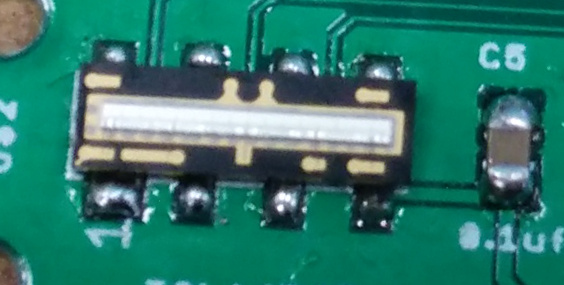
\includegraphics[width=0.5\textwidth]{images/sensor/IMG_20150414_135533_.jpg}
    \caption[Sensor CCD lineal.]{En la Figura apreciamos el sensor CCD que es capaz de captar luces que inciden sobre él}
    \label{fig:sens_CCD}
\end{figure}

Se realiza el pedido a la empresa Mouser, que es un distribuidor de componentes electrónicos, con el siguiente material.

\begin{table}[H]
    \centering
    \begin{tabular}{cc}
        {\bf Descripción}                 & {\bf Cantidad} \\ \hline
        Condensador cerámico SMD $0.1 \mu F$ & 2              \\
        Condensador cerámico SMD $1 \mu F$   & 2              \\
        Condensador cerámico SMD $10 \mu F$  & 1              \\
        LED Trough hole Rojo             & 1              \\
        LED SMD Rojo                     & 1              \\
        Resistencia SMD 1/8 WAT 150ohms  & 1              \\
        Resistencia SMD 1/8 WAT 300ohms  & 1              \\
        Resistencia SMD 1/8 WAT 1Kohms   & 1              \\
        Pulsadores SMD                   & 1              \\
        8bit Microcontrolador Freescale  & 1              \\
        Sensor CCD 1x128 pixeles         & 1             
    \end{tabular}
    \caption{BOM sensor de diámetro}
    \label{tab:BOM}
\end{table}

Para conseguir la PCB se usan los ficheros gerber disponibles en la web del proyecto \cite{thing_filamento}. Los ficheros gerber, contienen la información necesaria para la fabricación de la placa de circuito impreso.

\begin{figure}[H]
    \centering
    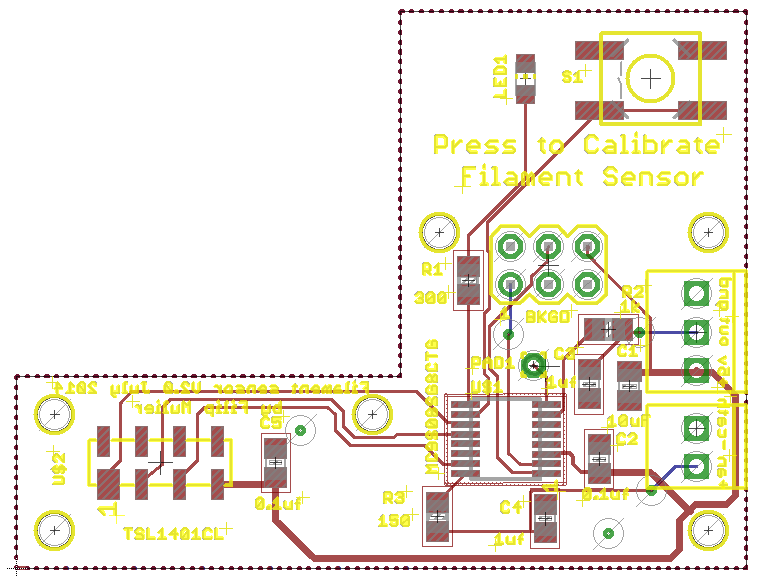
\includegraphics[width=0.5\textwidth]{images/sensor/gerber.png}
    \caption{Fichero gerber de la pcb.}
    \label{fig:sens_gerber}
\end{figure}

La única manera de realizar las PCB que disponemos es encargándola por Internet \footnote{http://www.seeedstudio.com/depot/}. Enviamos los gerber y tras establecer las especificaciones de la PCB en unos días recibimos el pedido.\\
\begin{figure}[H]
    \centering
    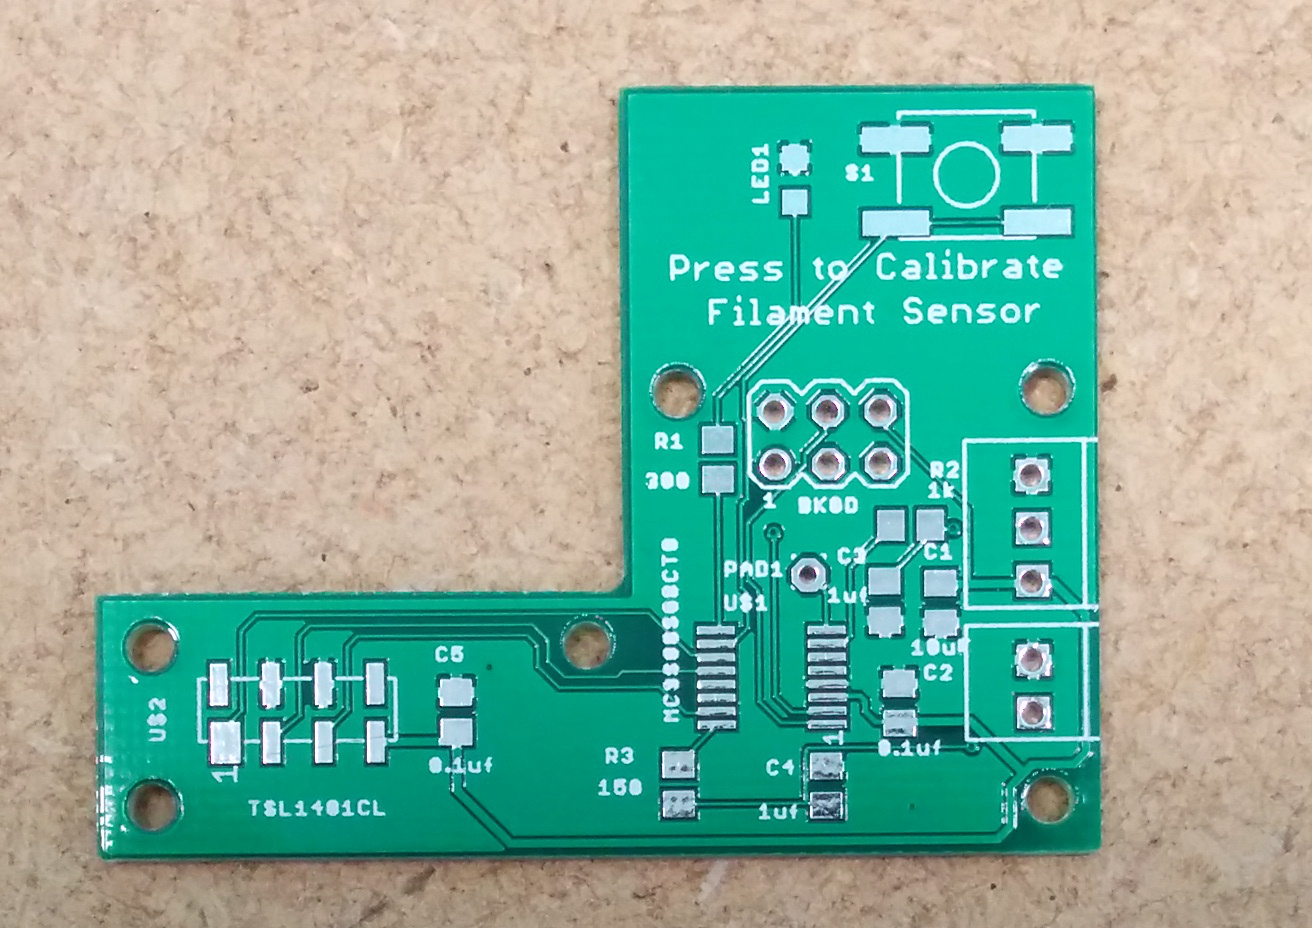
\includegraphics[width=0.5\textwidth]{images/sensor/IMG_20150414_105219_.jpg}
    \caption{PCB ya fabricada.}
    \label{fig:sens_pcb}
\end{figure}

El siguiente paso será soldar todos los componentes. En este caso, la mayoría de los componentes son de montaje superficial (SMD) por ello necesitaremos el siguiente material, para que la soldadura sea más fácil.

\begin{itemize}
	\item{Soldador.}
	\item{Estaño fino.}
	\item{Flux.}
	\item{Pinzas de punta fina.}
\end{itemize}

\begin{figure}[H]
    \centering
    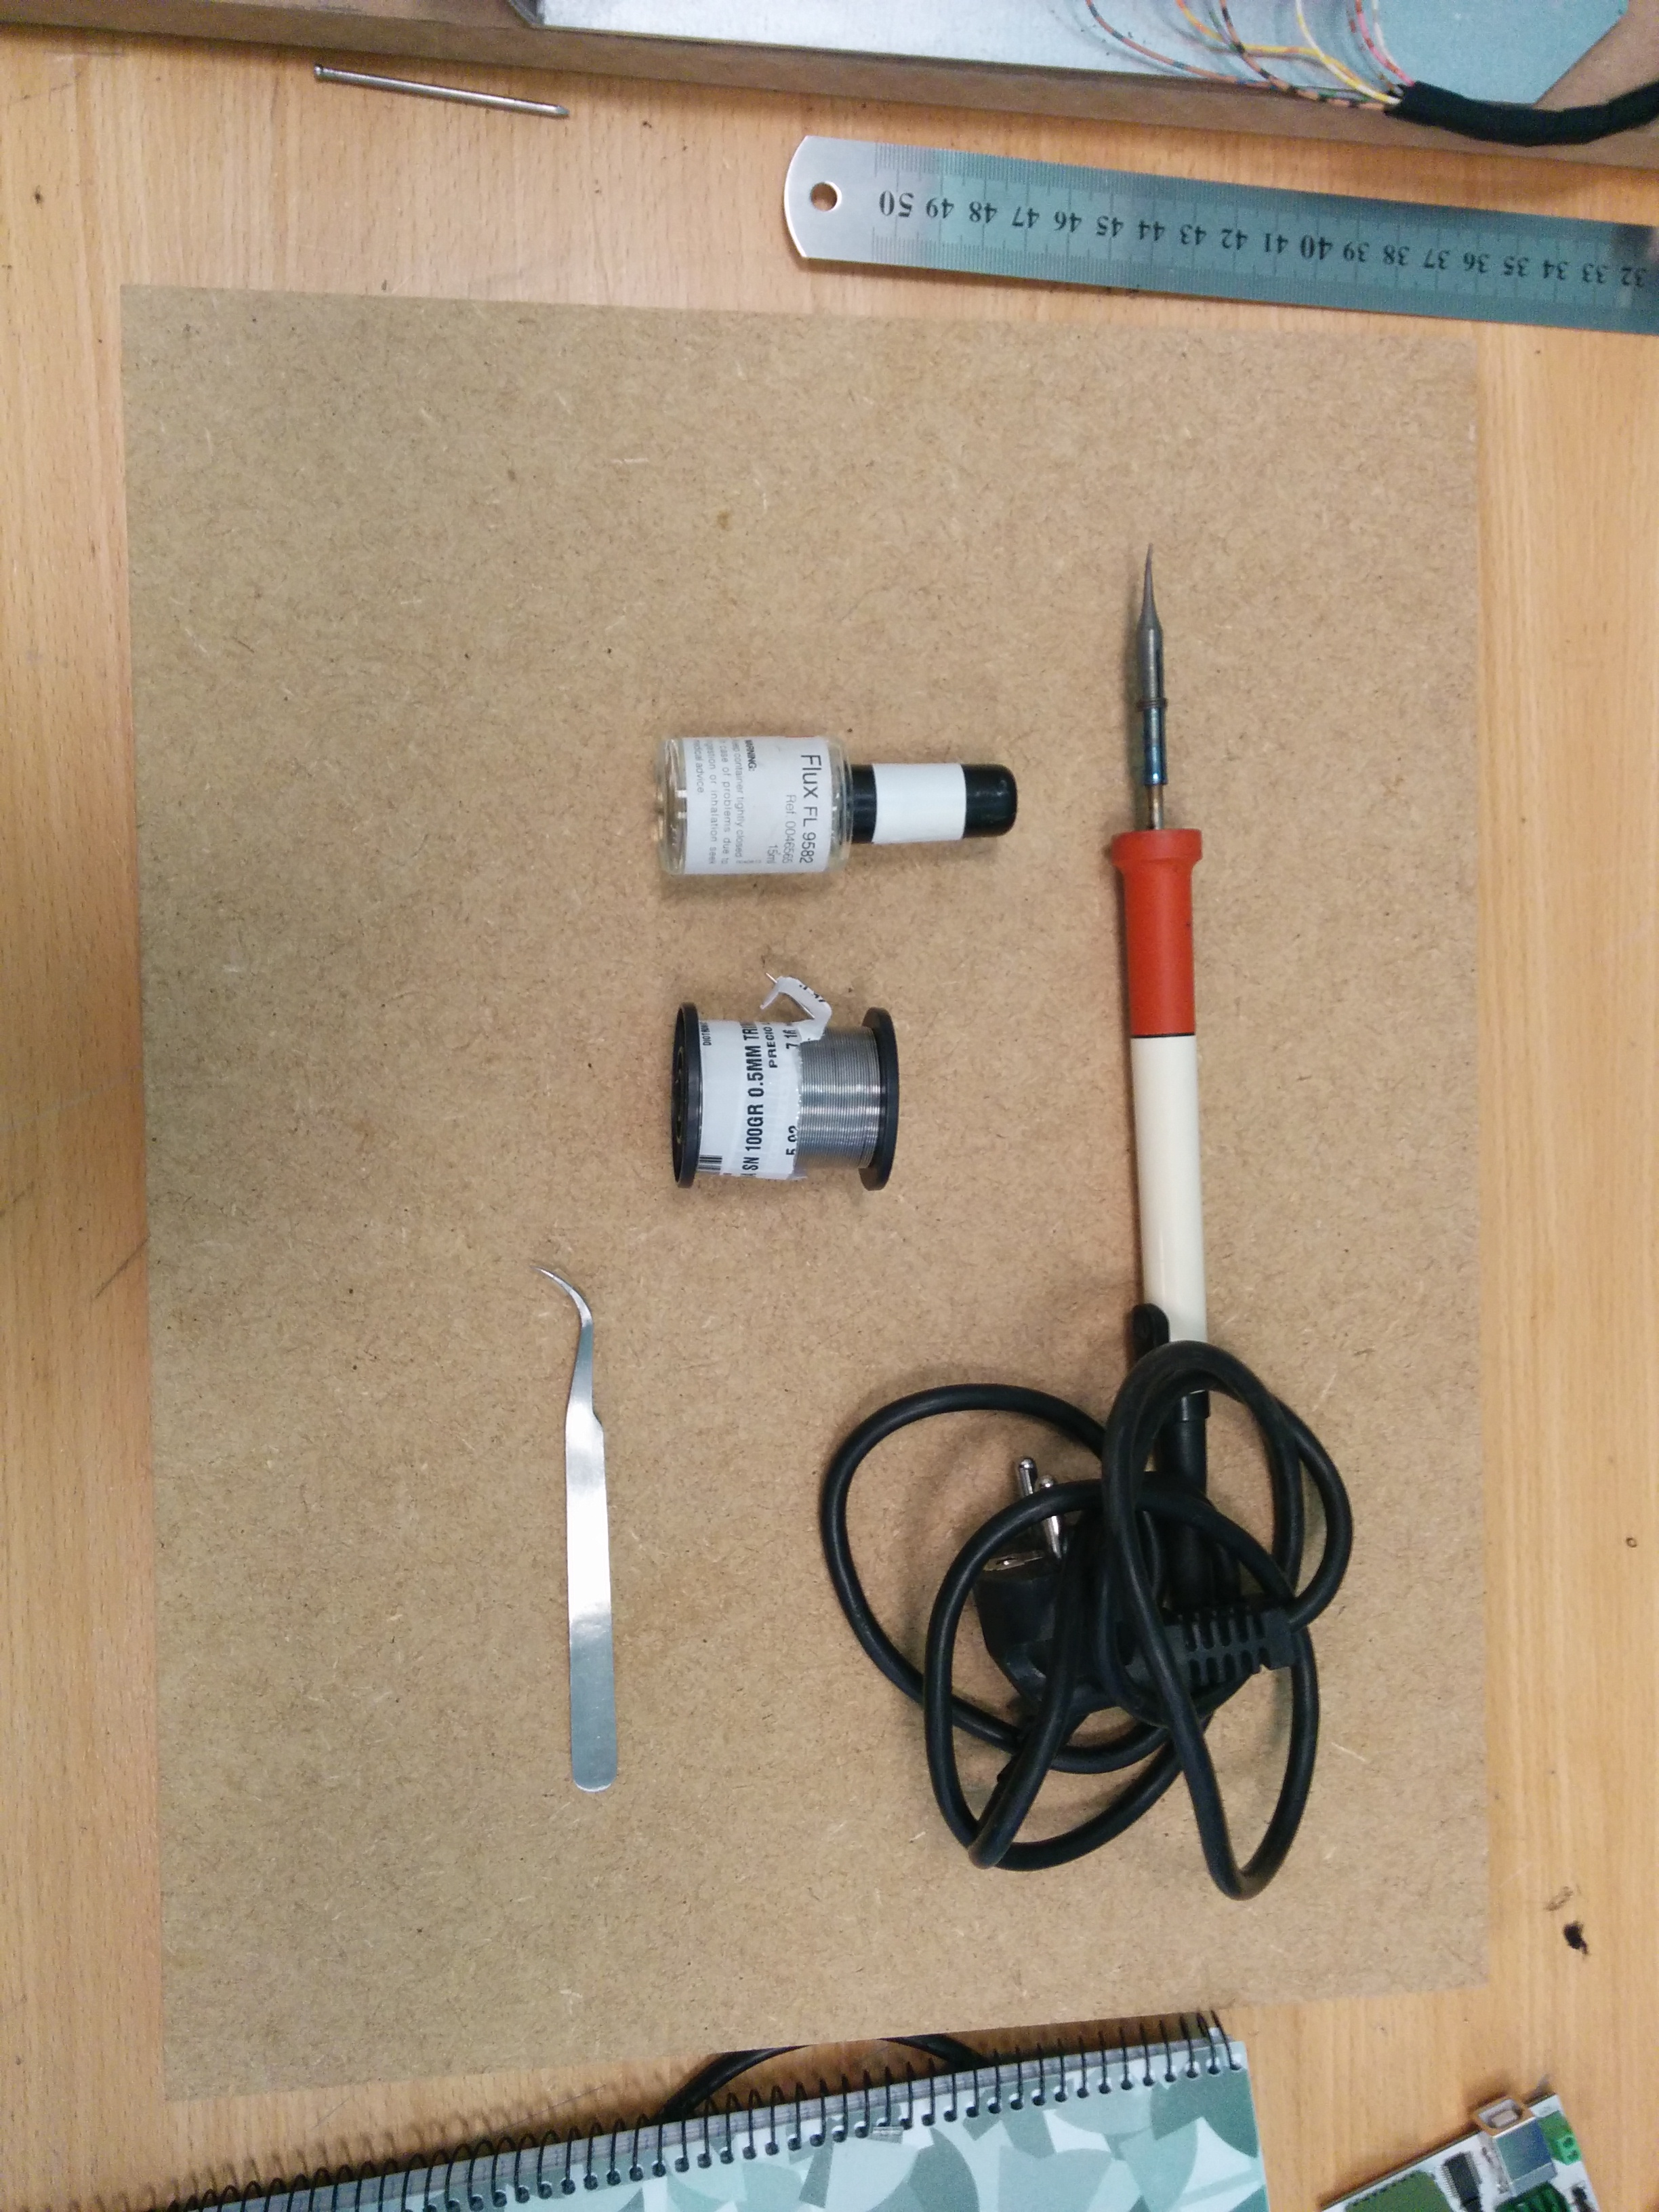
\includegraphics[width=0.5\textwidth]{images/sensor/IMG_20150417_160216.jpg}
    \caption{Materiales necesarios para soldar}
    \label{fig:sens_materiales}
\end{figure}

El componente más complicado de soldar es el microcontrolador ya que tiene sus pines muy cercanos entre sí. Para evitar que el estaño cortocircuite dos pines, se esparcirá Flux que es un líquido que ayuda a la hora de soldar, limpiando la superficie y haciendo que  el estaño sea más fácil de fundir.\\
\begin{figure}[H]
    \centering
    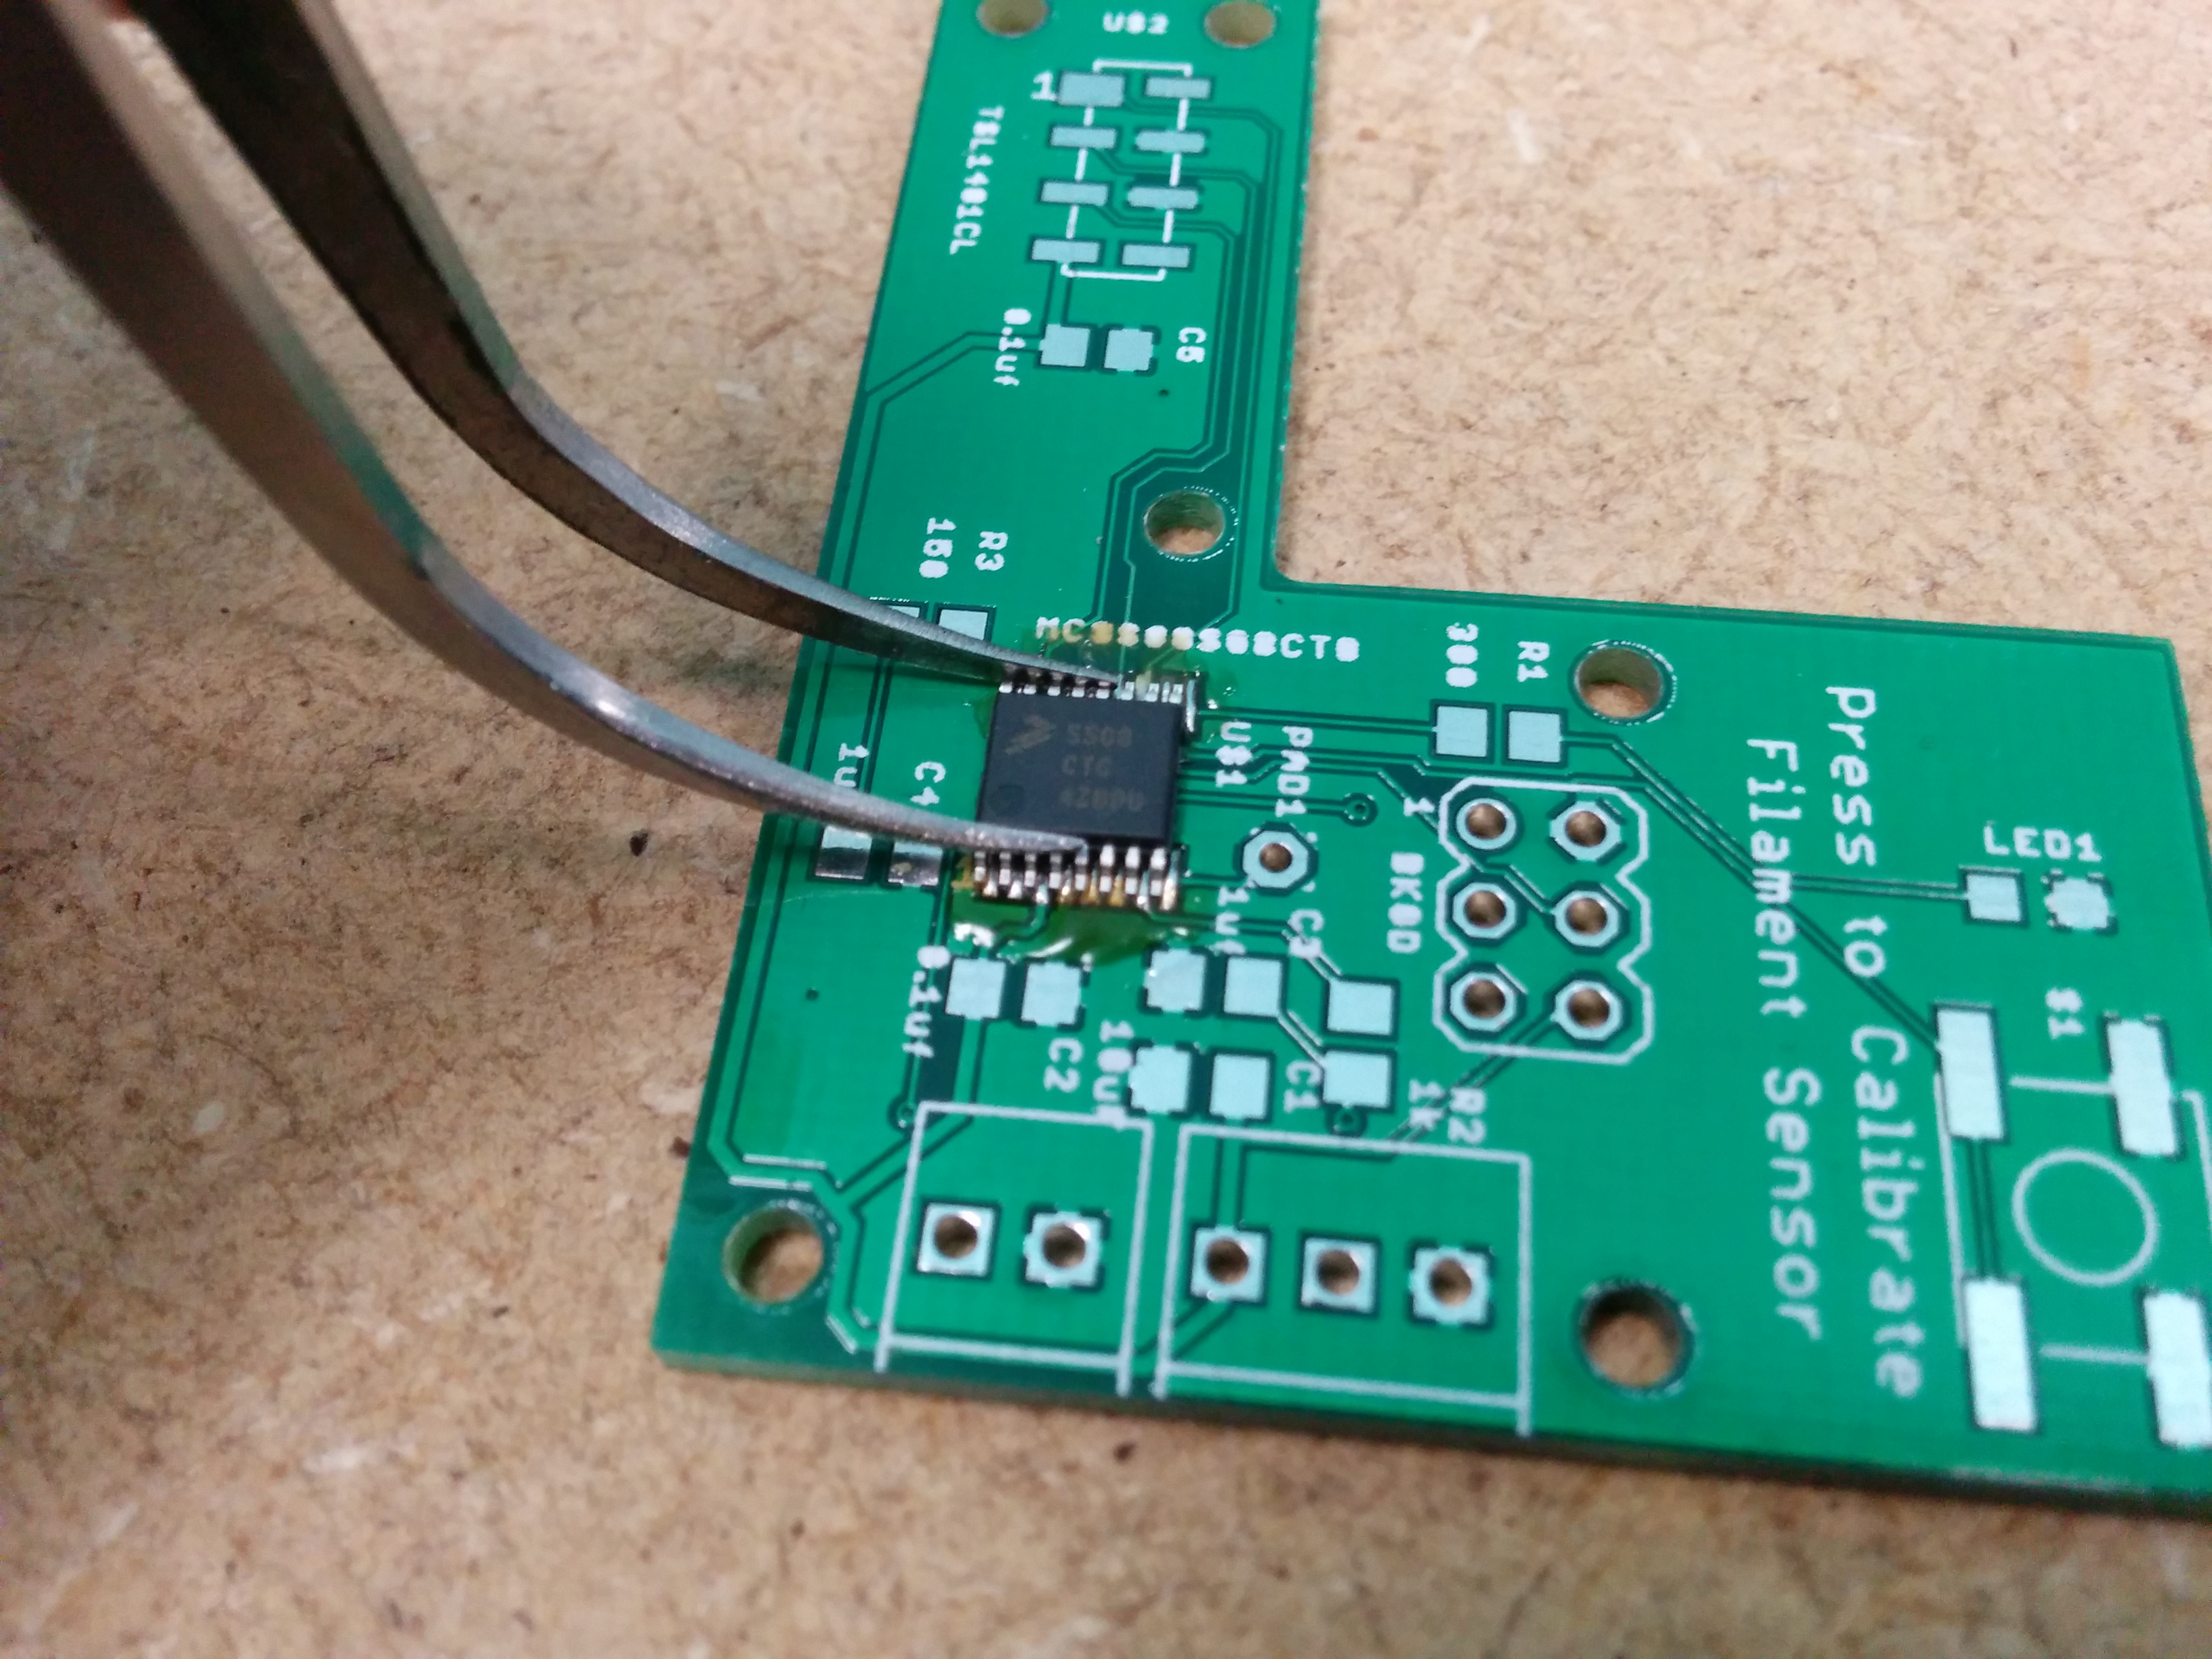
\includegraphics[width=0.5\textwidth]{images/sensor/IMG_20150414_111135.jpg}
    \caption{Soldando el microcontrolador.}
    \label{fig:sens_micro}
\end{figure}

El resto de componentes SMD son fáciles de soldar y con ayuda de la pinza se irán soldando en orden.
\begin{figure}[H]
    \centering
    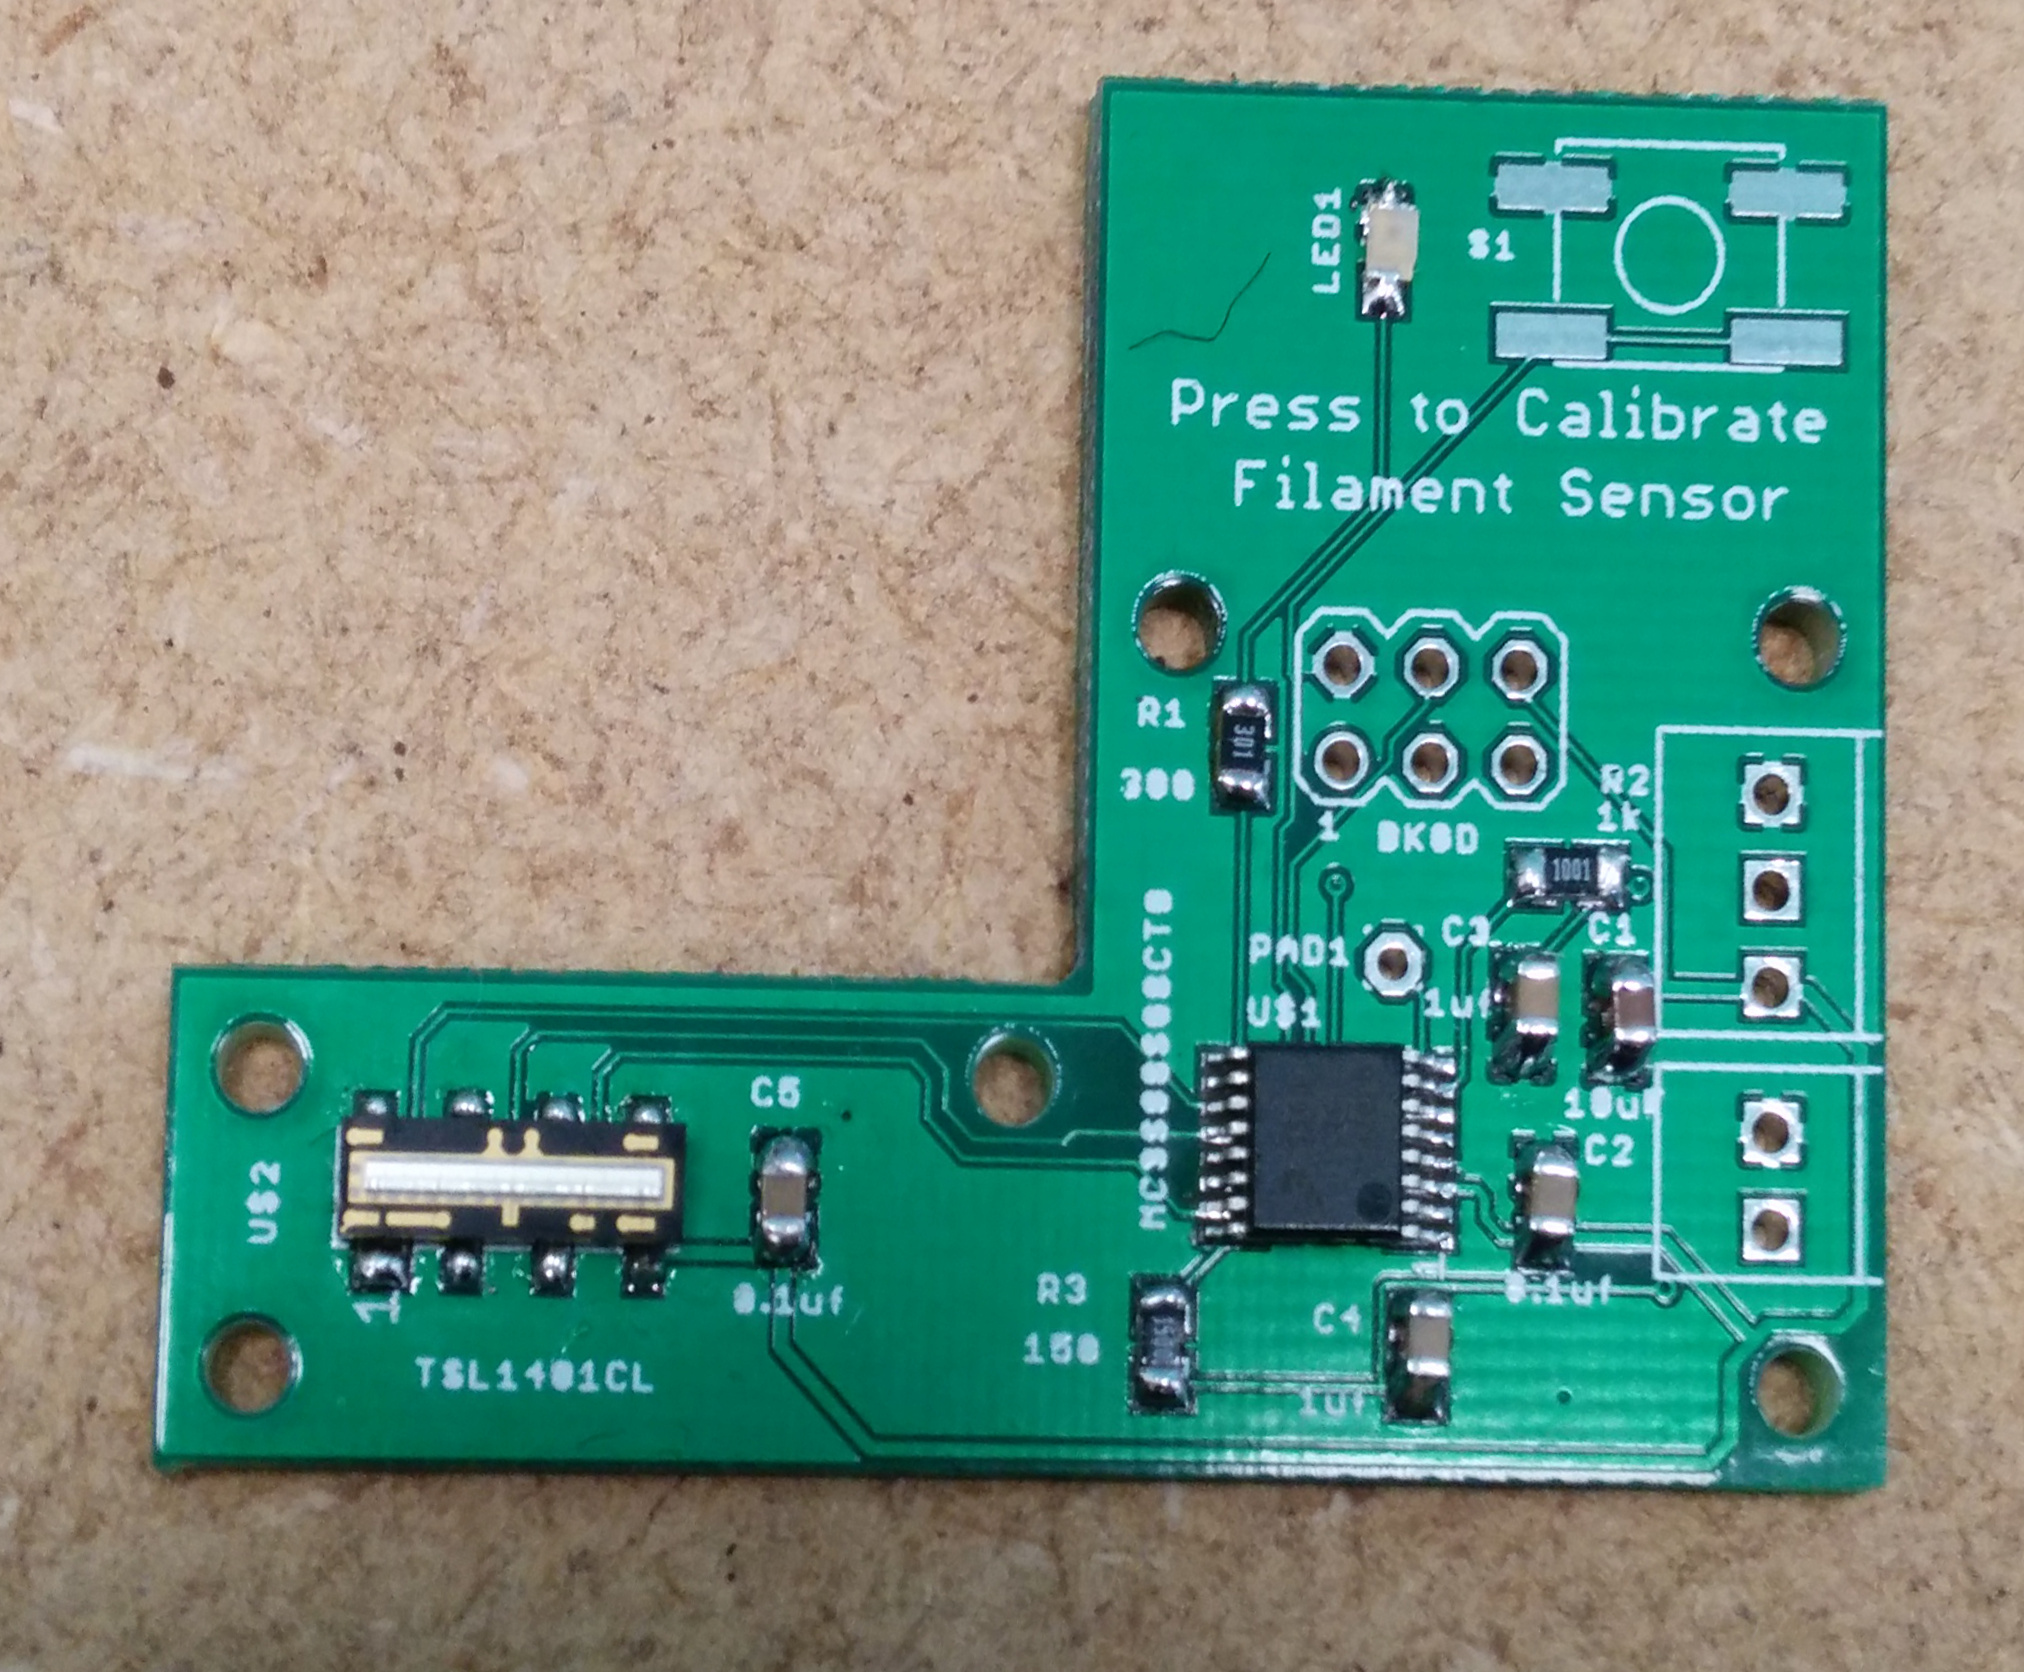
\includegraphics[width=0.4\textwidth]{images/sensor/IMG_20150414_135533.jpg}
    \caption{Soldando componentes SMD.}
    \label{fig:sens_SMD}
\end{figure}
Los últimos componentes a soldar serán los que atraviesen la placa de circuito impreso con sus pines (Trough hole) terminando así de soldar todos los componentes:\\
\begin{figure}[H]
    \centering
    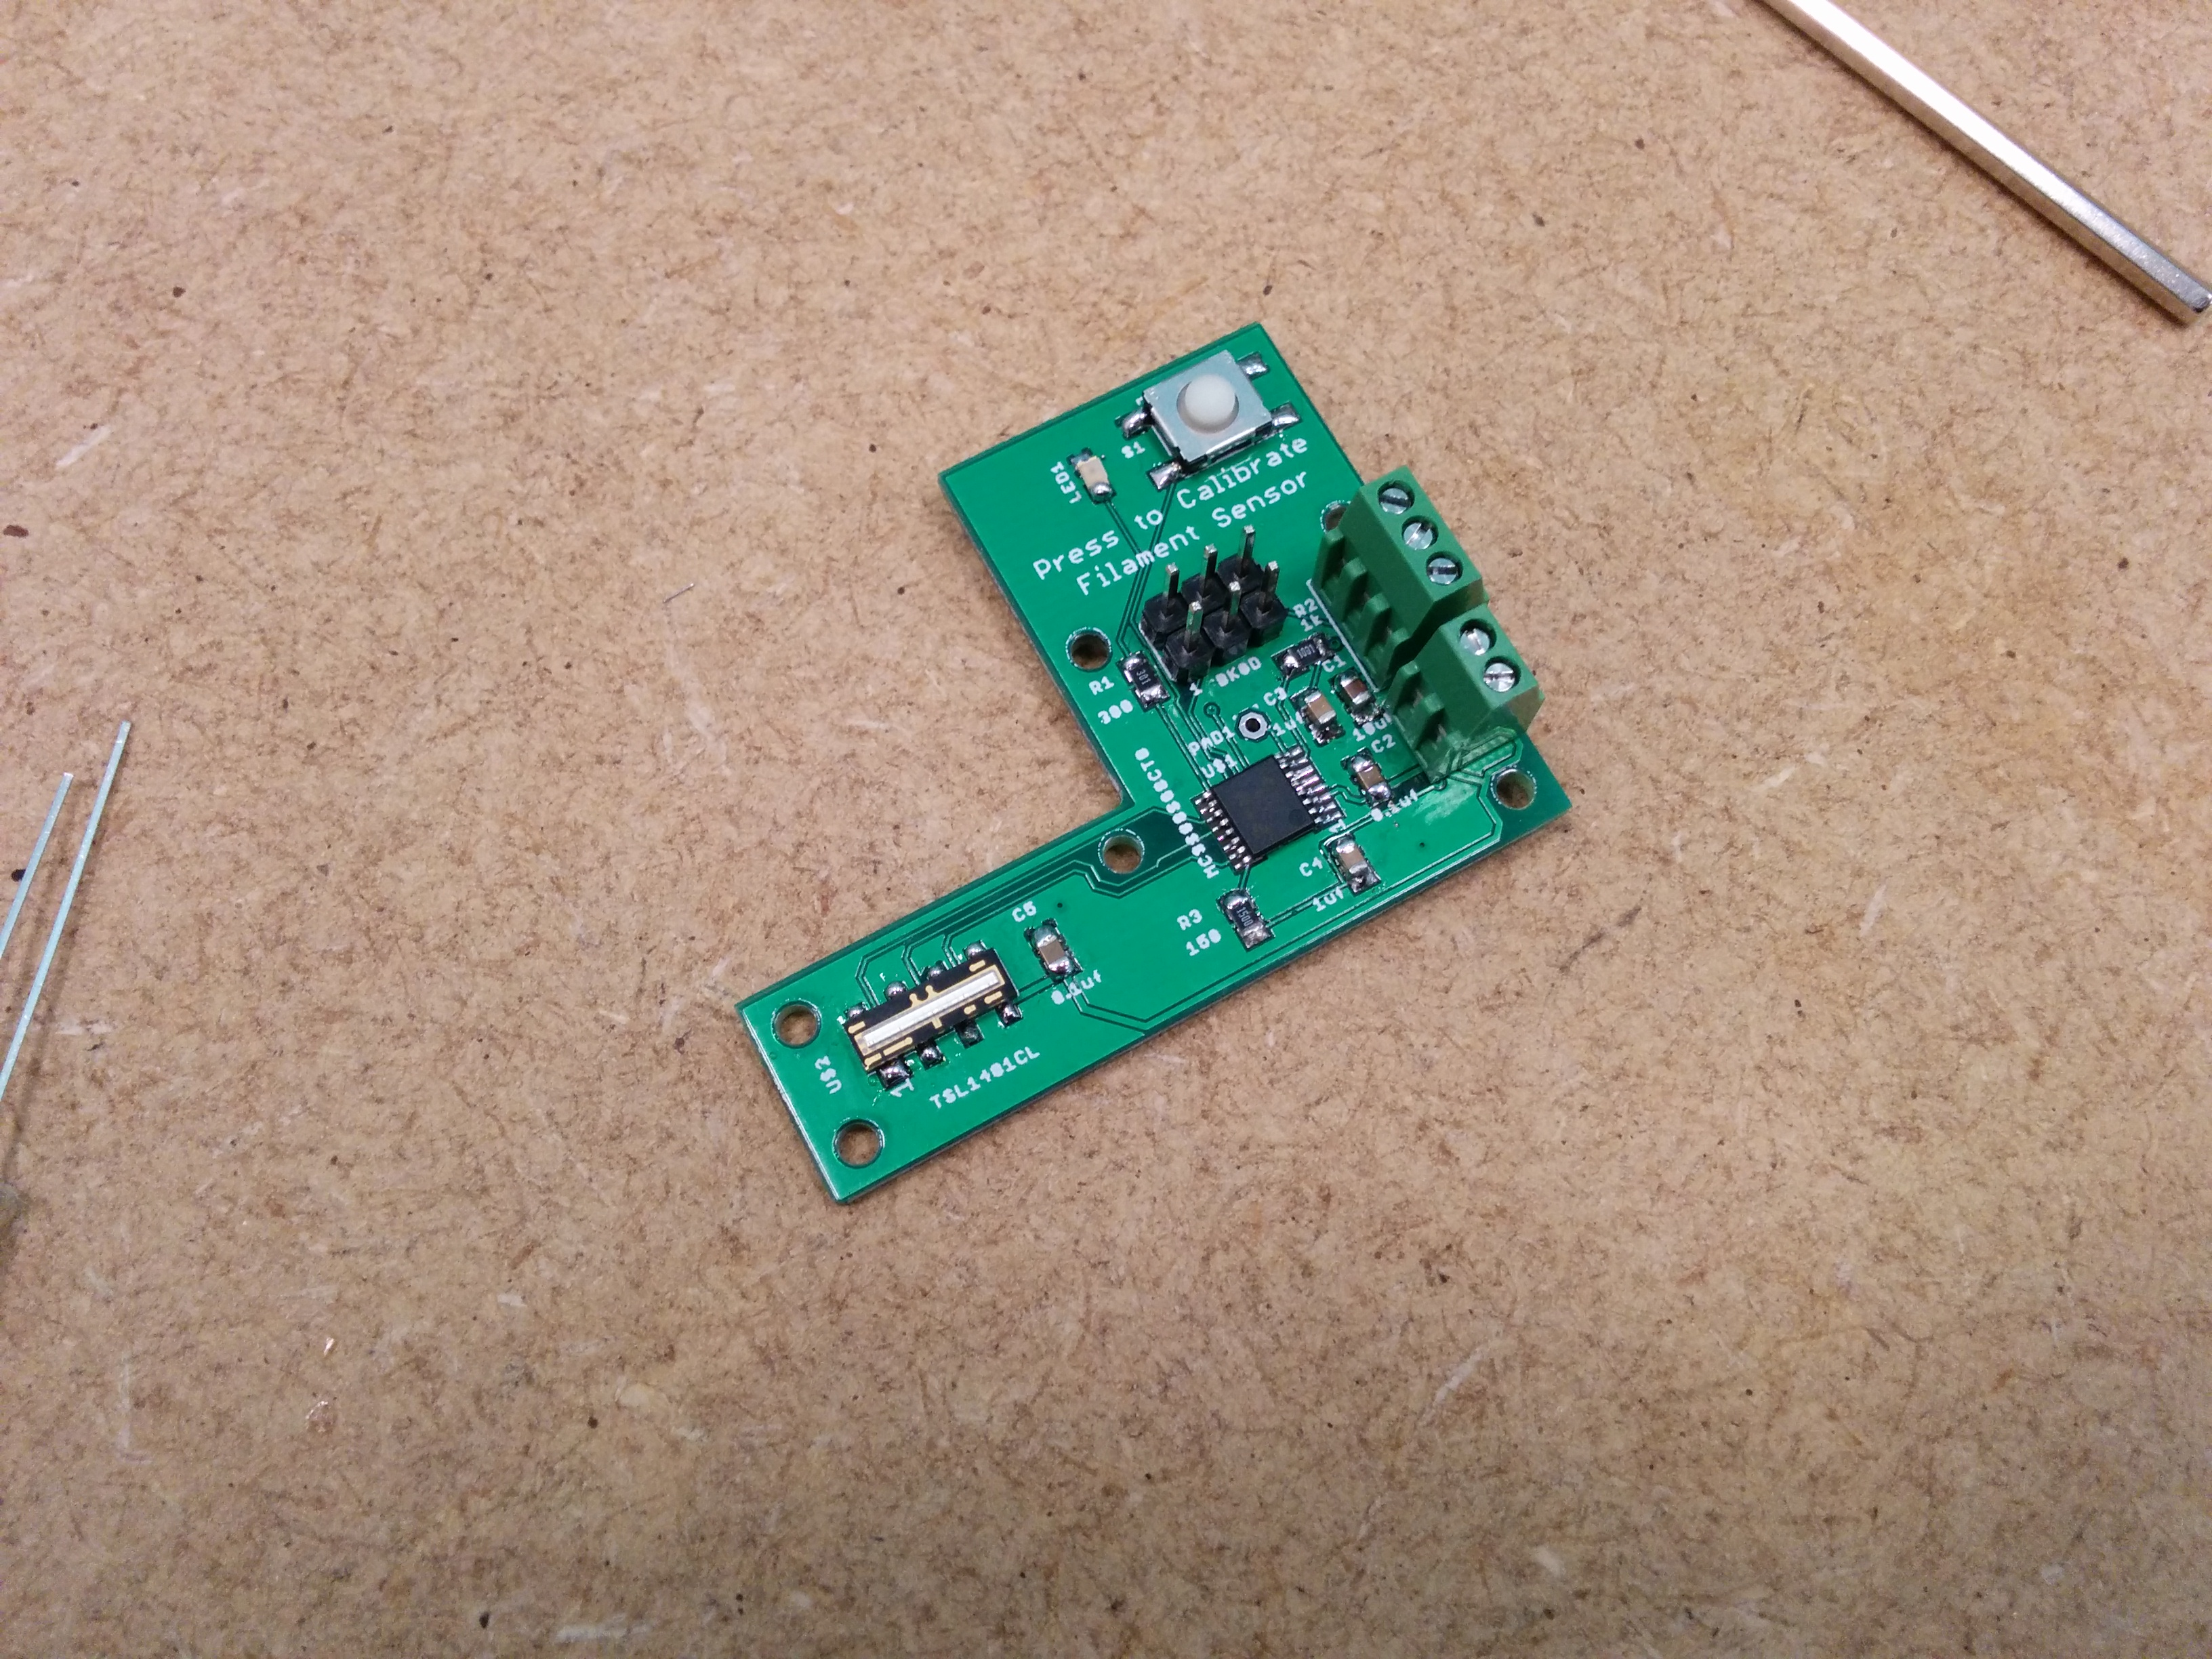
\includegraphics[width=0.5\textwidth]{images/sensor/IMG_20150417_121941.jpg}
    \caption{Placa con los componentes soldados.}
    \label{fig:sens_SMD2}
\end{figure}

Por último, programaremos el microcontrolador con el firmware que nos bajamos e introduciremos la PCB ya soldada, en una carcasa de plástico que imprimimos con ayuda de una impresora 3D.
\begin{figure}[H]
    \centering
    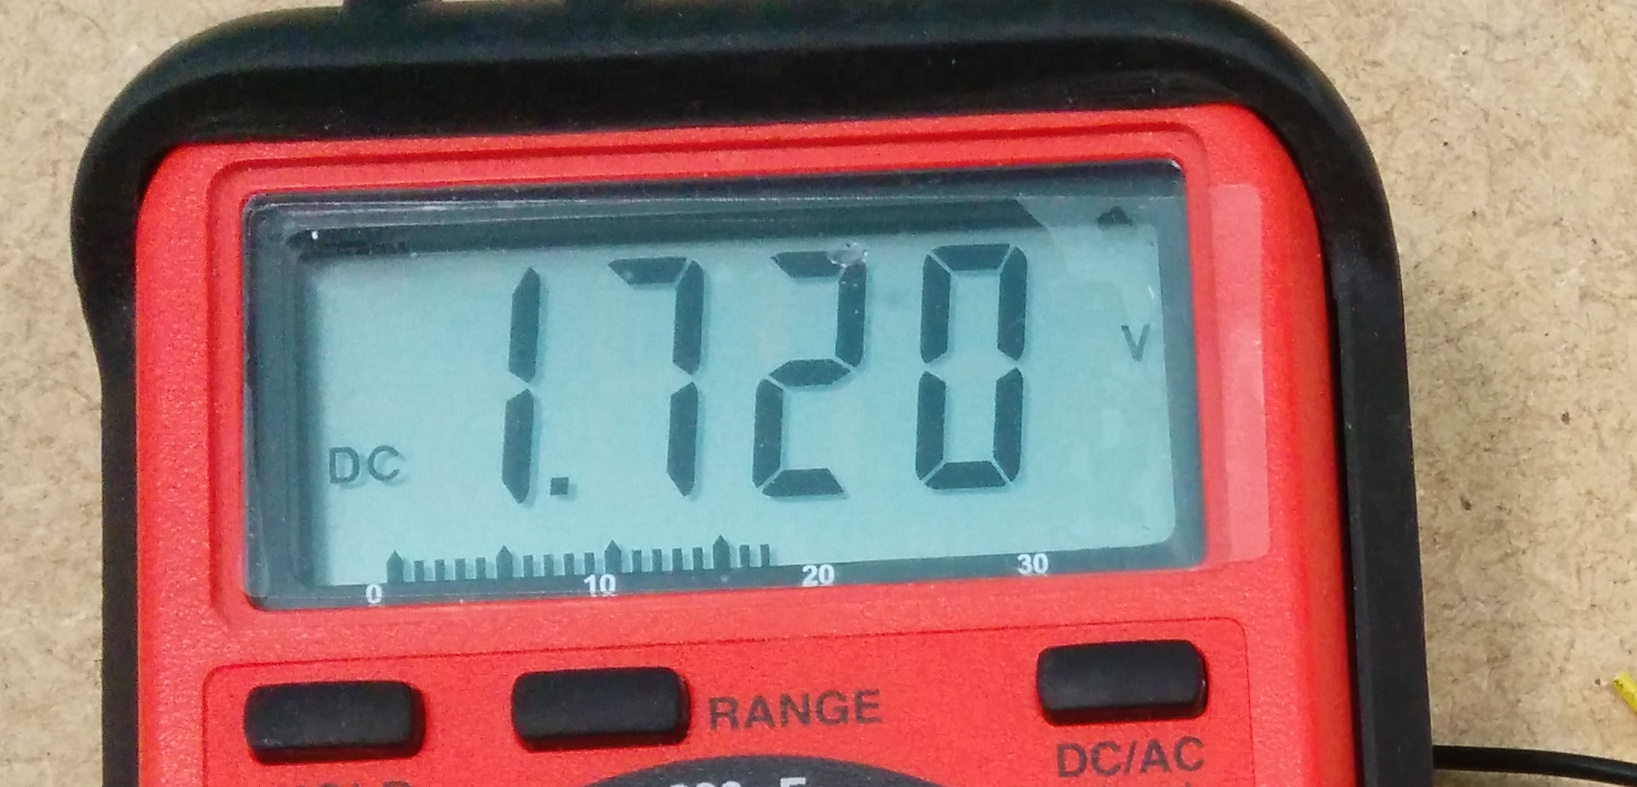
\includegraphics[width=0.5\textwidth]{images/sensor/IMG_20150417_134451.jpg}
    \caption{Sensor midiendo un filamento de 1.75mm.}
    \label{fig:sens_midiendo}
\end{figure}

Al realizar varias medidas, se comprueba que se comete un ligero error en la medida, y eso es debido a que a la hora de calibrar no disponemos de un varilla con la misma medida con la que el usuario realizó la programación. Después de realizar unas mediciones con el sensor de unas dimensiones conocidas, estos son los valores obtenidos.\\

\begin{table}[H]
    \centering

    \begin{tabular}{cc}
        {\bf Voltaje (V)} & {\bf Diametro real(mm)} \\ \hline
        0                 & 0                       \\
        1,13              & 1,14                    \\
        1,56              & 1,57                    \\
        1,82              & 1,82                    \\
        1,93              & 1,94                    \\
        2,37              & 2,36                    \\
        2,77              & 2,74                   
    \end{tabular}
    \caption{Mediciones con el sensor.}
    \label{tab:medici_senso}
\end{table}

Como comprobamos en la tabla \ref{tab:medici_senso} se comete un error en cada medida, por ello, se realiza una regresión lineal para intentar minimizar el error cometido.

\begin{figure}[H]
    \centering
    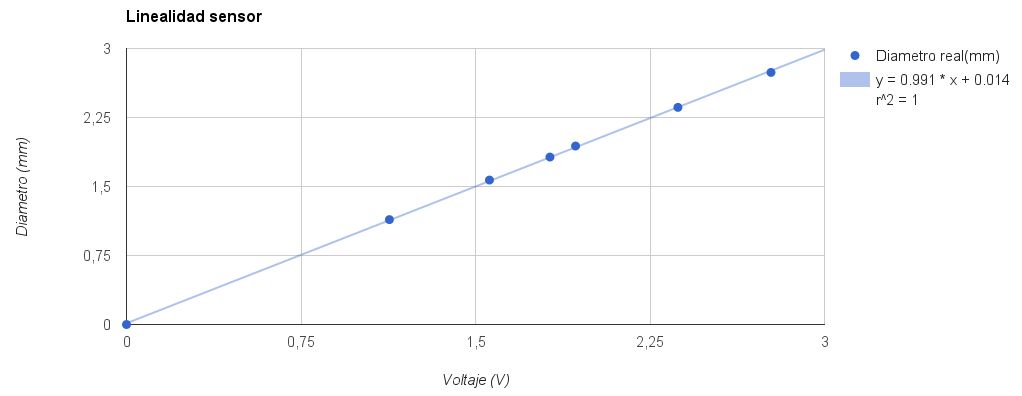
\includegraphics[width=0.9\textwidth]{images/sensor/linealidad_sensor.png}
    \caption[Gráfica con regresión lineal.]{Gráfica con regresión lineal. Vemos la linealidad del sensor y como ajustando la recta por mínimos cuadrados podemos corregir la pequeña desviación que existe.}
    \label{fig:sens_regre}
\end{figure}

La ecuación de la recta que minimiza el error en la medición es:
$$y= 0.991*x +0.015$$